\section{Training Schedule And Assignments}
\subsection{Training Schedule By Month For The Entire Training Period}
The training schedule is depicted in Table \ref{tab:schedule} below. This schedule was developed by my supervisor, and is a rough guideline at best as the objectives of the company are evolving.
As such there may be important tasks that crop up that I may require my attention.
\begin{table}[h!]
	\caption{Training Schedule}
	\label{tab:schedule}
	\begin{tabularx}{\textwidth}{X|X|X}
		\multicolumn{1}{>{\centering}c|}{\textbf{Task}} & \multicolumn{1}{>{\centering}c|}{\textbf{Metric}} & \multicolumn{1}{c}{\textbf{Month}} \\
		\hline
		Familiarise with VueJS and Firebase \newline Start developing Inventory Management System (IMS) in the Lemon Dashboard & Integrate User Interface with backend & Jan\\
		Continue Development of IMS and conduct developer testing  & Accuracy of Lemon IMS flow based on given Requirements & Feb\\
		Working on backend to track earnings of drivers involved in Lemon earnings & Accuracy of payment flow & Mar\\
		Integration Testing of Lemon Dashboard with other platforms such as Mobile & Robustness and latency & Apr\\
		Collect user feedback from pre-pilot trial and work on improving the dashboard & Speed and responsiveness & May\\
		Deploy using Docker and open-source CI/CD system & Robustness & Jun\\
	\end{tabularx}
\end{table}

\subsection{Training Assignments Completed in 1st Month}
My first task for the month was to familiarise with VueJS and Firebase. This was a manageable task as
I had previous experience in Javascript and Backend-as-a-service (BaaS) tools such as Firebase. The main takeaways from
the Udemy course was routing, authentication, state management and design patterns in VueJS. It also introduced me to the 
Model-View-ViewModel (MVVM) Software Architechture that that the framework uses. With the help of the course, I built a simple
video browsing application that uses YouTube's API, as shown in Figure 1.

\begin{figure}[h!]
	\begin{center}
		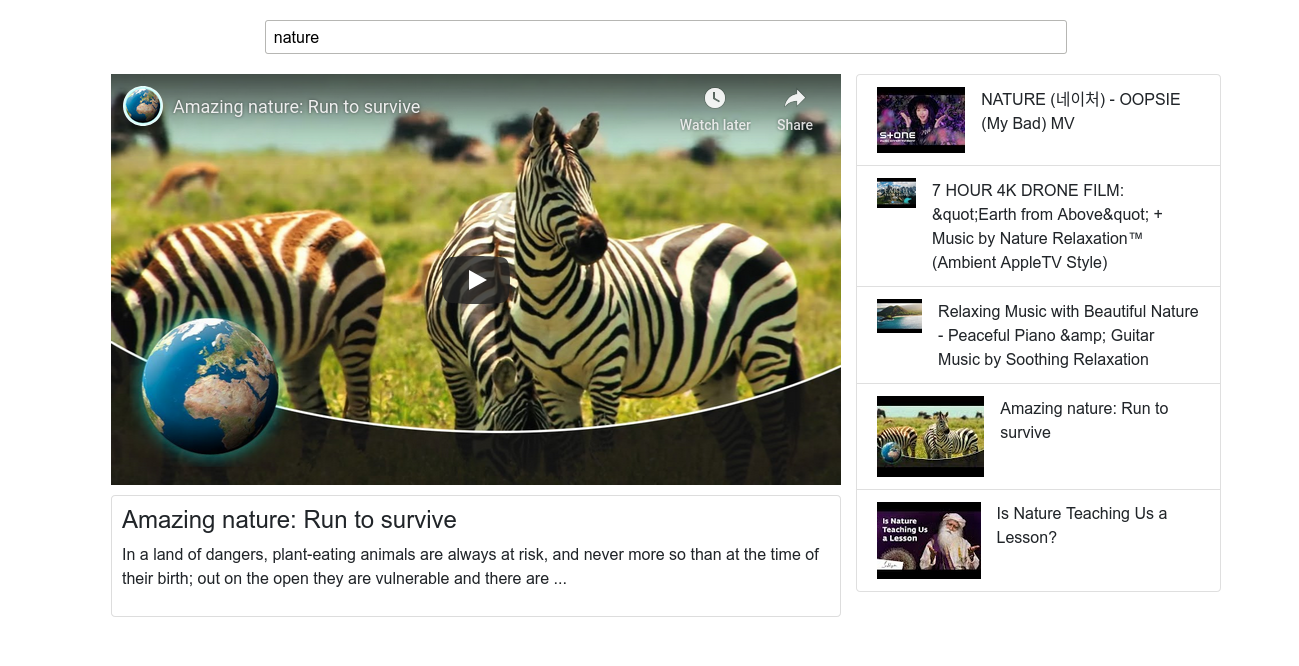
\includegraphics[width=350px]{assets/images/udemy-project.png}
		\caption{Video browsing application}
		\label{fig:govsg-chatbot}
	\end{center}
\end{figure}

\pagebreak

\noindent
Subsequently, I started work on the Inventory Management System (IMS) for the Lemon Project. This constituted
developing the user interface to help administrators perform create, read, update and delete (CRUD) operations
for inventory items as shown in Figure 2. As such I also began interacting with the Database to perform the CRUD operations.

\begin{figure}[h!]
	\begin{center}
		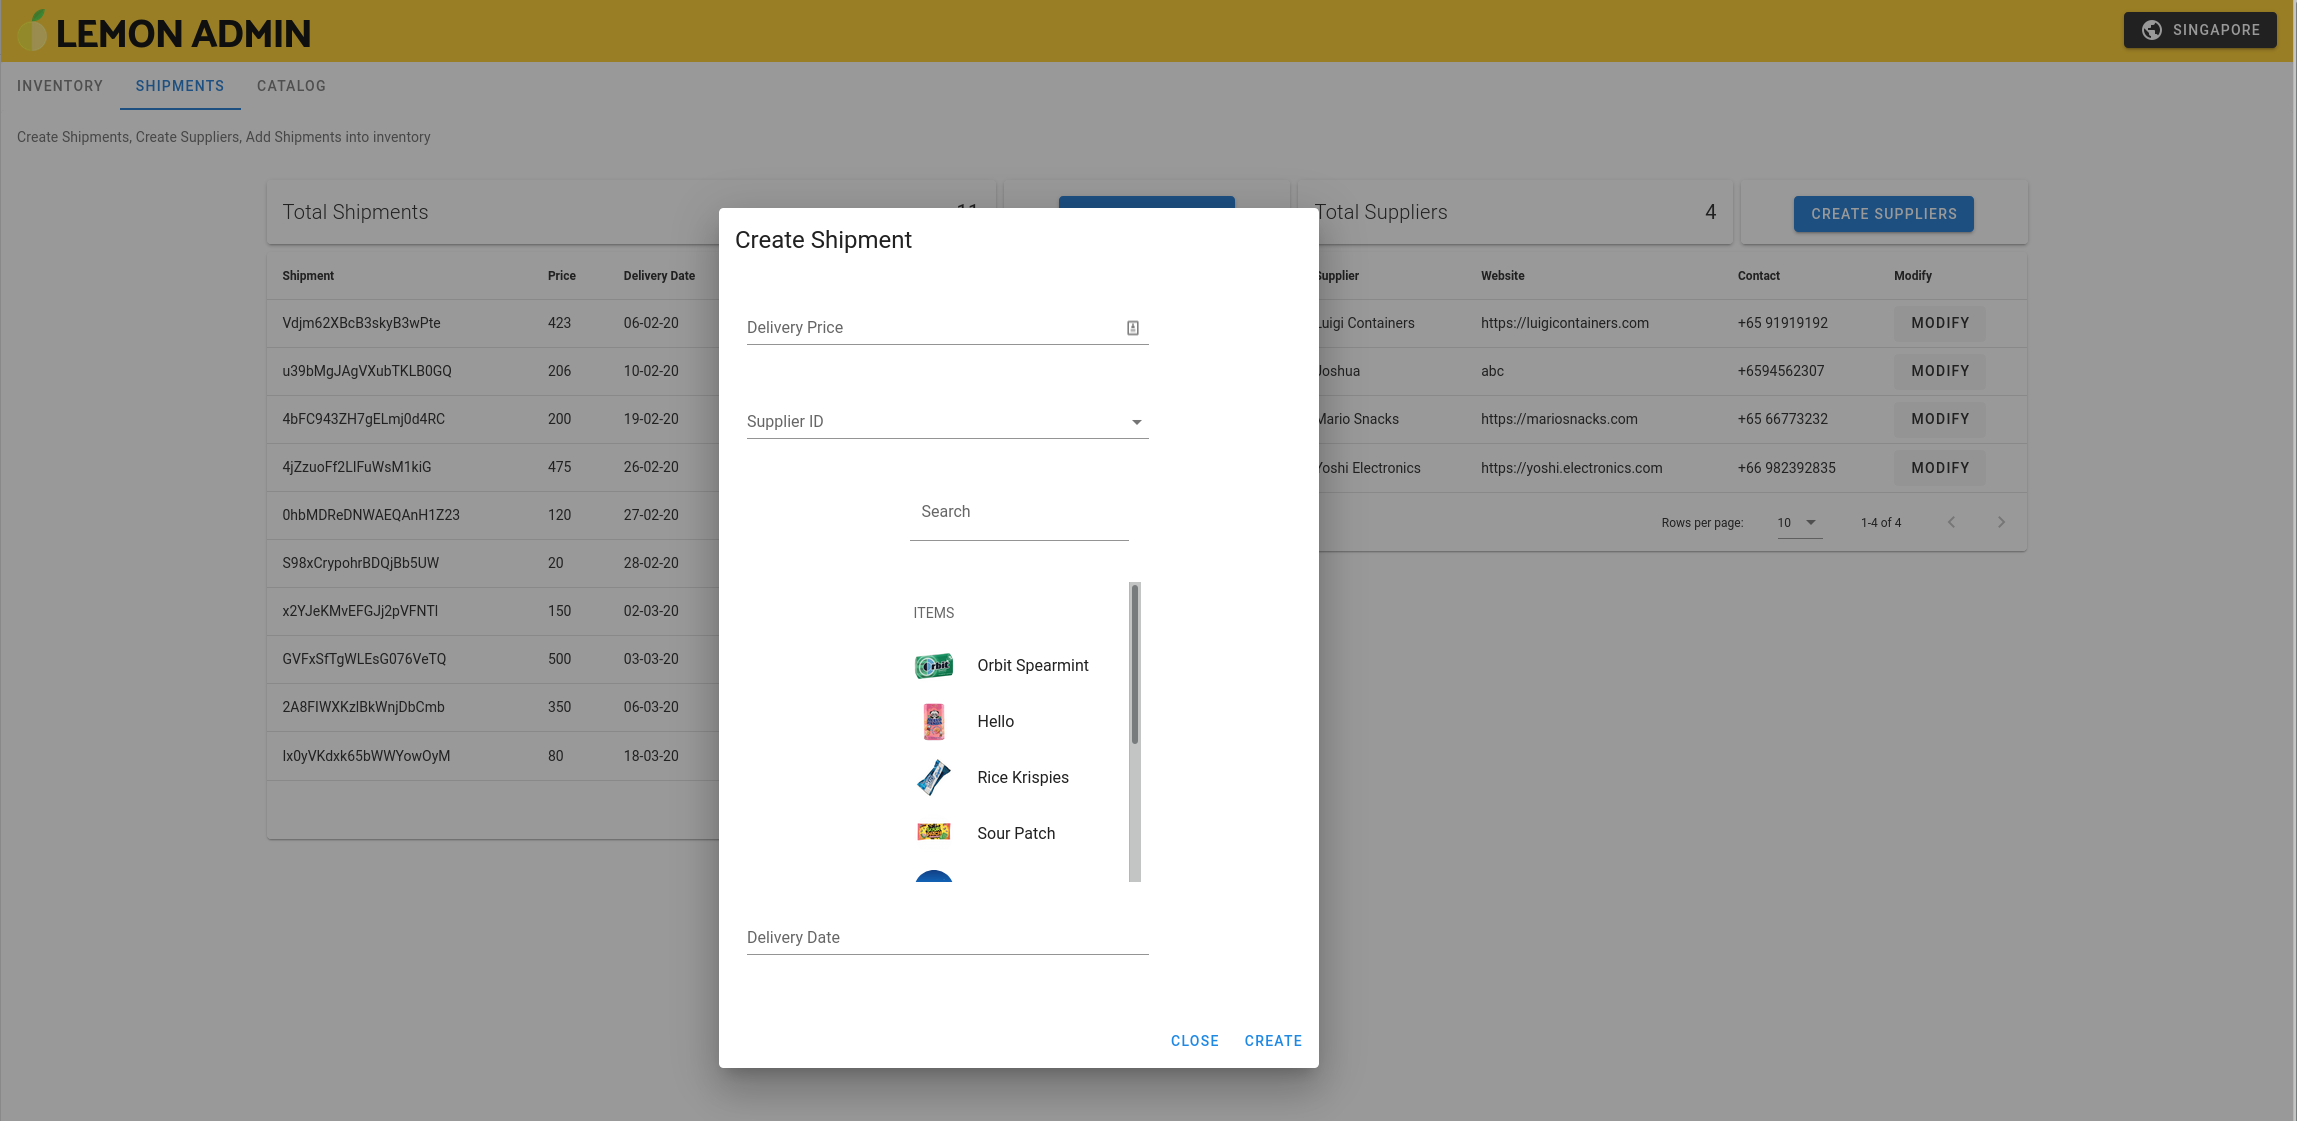
\includegraphics[width=350px]{assets/images/lemon-shipment.png}
		\caption{Inventory Management System: Shipments and Suppliers}
		\label{fig:lemon-shipment}
	\end{center}
\end{figure}

\subsection{Training Assignments Completed in 2nd Month}
\noindent
In this month, I continued my main task of developing the IMS. I completed work on integrating Suppliers, Shipments and Inventory to the IMS as shown in Figure 3.
The increasing complexity of the code base helped me improve important web development techniques such as introducing asynchronous programming and a more advanced state management pattern.\cite{REF2:1} 

\begin{figure}[h!]
	\begin{center}
		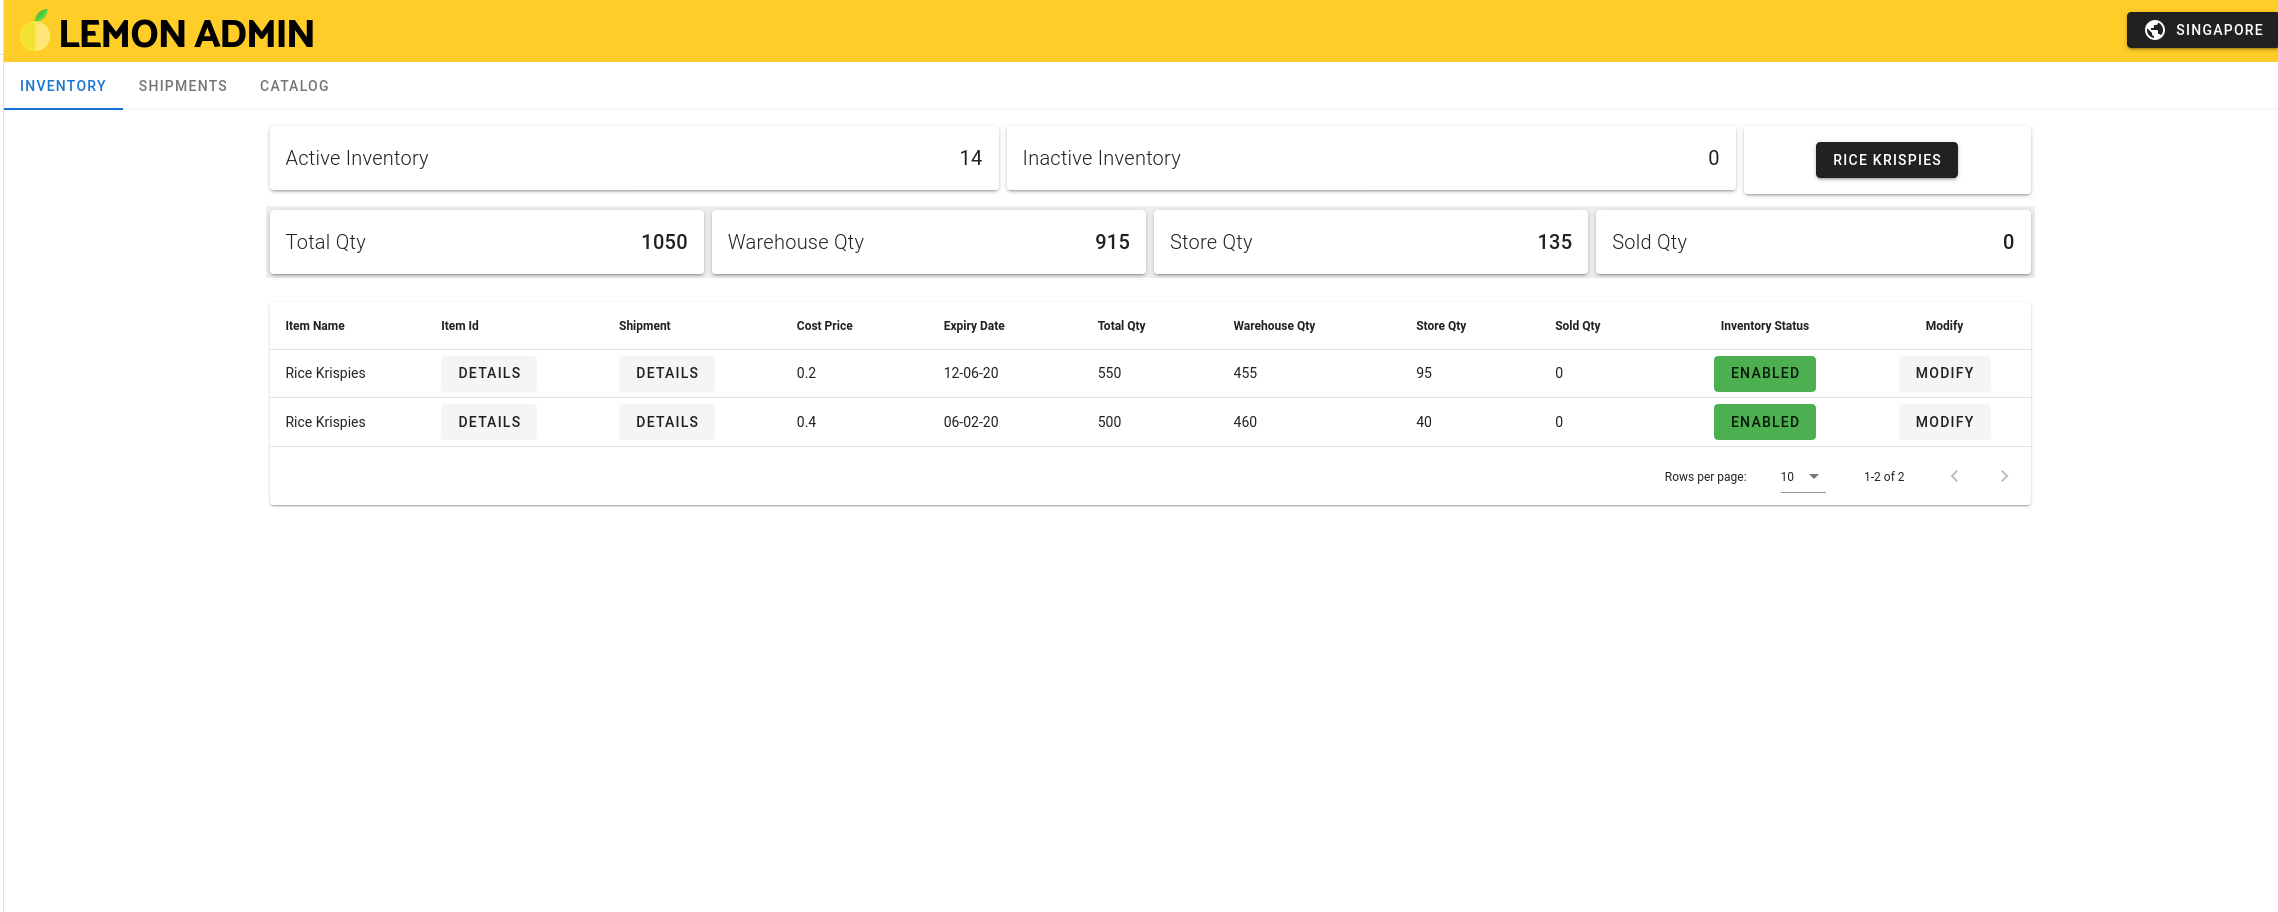
\includegraphics[width=350px]{assets/images/lemon-inventory.png}
		\caption{Inventory Management System: Inventory}
		\label{fig:lemon-inventory}
	\end{center}
\end{figure}

\noindent
My second main task was to perform developer testing for the IMS. Through developer testing, my supervisor and I discovered errors in the code where the behavior did not match the specifications in the requirements.
As such I performed bug fixes and deployed them as well. This process also helped me improve the efficiency in which the front-end
code manipulated the Domain Object Model (DOM).

\subsection{Training Assignments Completed in 3rd Month}
\noindent
One task I completed was working on the backend code in Node.JS for the payment flow. Drivers enrolled in Lemon's pilot programme are to be paid by the customers they hail. In the case of 
credit card payments, Lemon uses Stripe \cite{REF3:1} as its payment gateway to facilitate the payments. Stripe's Software Development Kit (SDK) uses Webhooks to perform actions
once payments are successful. I was expected to test these webhooks and ensure they behaved as expected in various situations users may experience.
\noindent
My supervisor also tasked me with optimising the payment flow, such as improving error handling, and
updating driver earnings (Figure 4), after each successful cash or credit card payment. Subsequently, the backend code was deployed to Firebase.

\begin{figure}[h!]
	\begin{center}
		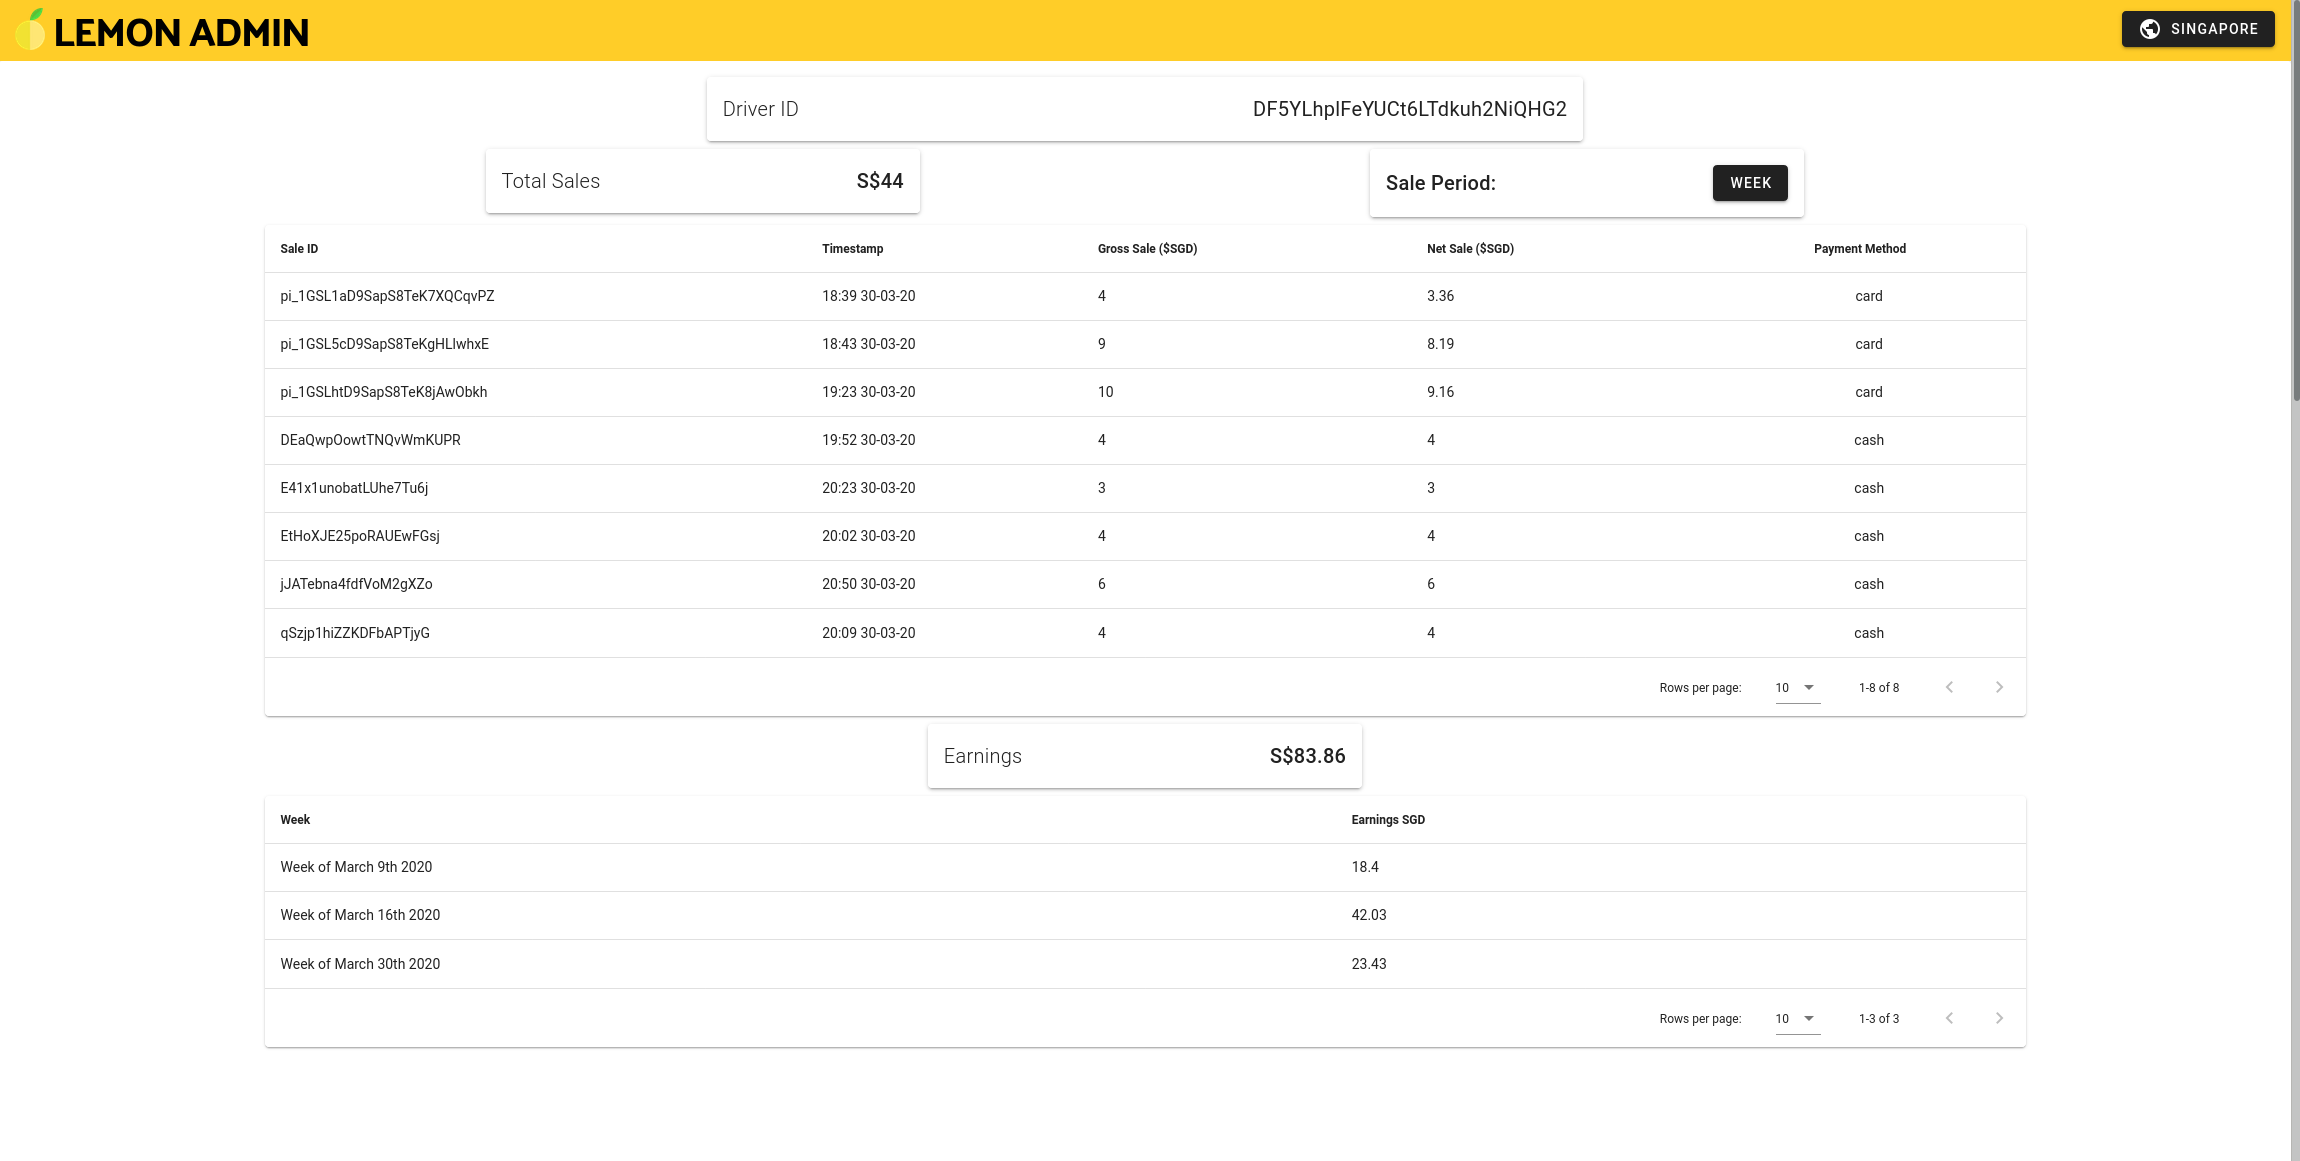
\includegraphics[width=350px]{assets/images/lemon-earnings.png}
		\caption{Driver earnings UI}
		\label{fig:lemon-earnings}
	\end{center}
\end{figure}

\noindent
Another task I completed was securing the Database. I wrote Firebase security rules to ensure that certain collections in the NoSQL Database collection tree prevented unauthenticated users from writing to them. This was imperative for the pilot trial of the system.